\documentclass{article} % For LaTeX2e
\usepackage[utf8]{inputenc}
\usepackage{cos424,times}
\usepackage{url}
\usepackage{graphicx}
\usepackage{amsmath}
\usepackage{amssymb}
\usepackage{float}
\usepackage{enumitem}
\usepackage{hyperref}

\graphicspath{{./figures/}} 

\newcommand{\R}{\mathbb{R}}
\newcommand{\D}{\mathbb{D}}
\newcommand{\I}{\mathbb{I}}
\DeclareMathOperator*{\argmax}{arg\,max}
\DeclareMathOperator*{\argmin}{arg\,min}
\usepackage{natbib}


\title{Prediction for Fragile Family Data}


\author{
Vivek Kumar\\
Civil and Environmental Engineering\\
Princeton University\\
\texttt{vivekk@princeton.edu} \\
\And
Victor Charpentier\\
Civil and Environmental Engineering\\
Princeton University\\
\texttt{vc6@princeton.edu} \\
}

\newcommand{\fix}{\marginpar{FIX}}
\newcommand{\new}{\marginpar{NEW}}

\begin{document}

\maketitle

\begin{abstract}
Applying machine learning techniques for social good is one of the bright outcomes of the technological revolution of the past years. In homework 2 we have performed a prediction and analysis of 6 key outcomes at age 15 of the fragile family challenge. The methods implemented depend on the type of outcome. For each type of outcome over 6 prediction methods are tested. The performance of regressions and classifiers is assessed with xx and receiver operating curves. Overall, the random forest regression methods has the best results for continuous variables. Finally, we determine the the important features and showcase how much error can be expected from the model.
\end{abstract}
\section{Introduction}
The fragile family challenge (FFC) is a Princeton University-led initiative opening the data collected in the long term Fragile Family and Child Wellbeing Study (FFCWS) to a variety of data scientists. The study follows an ensemble of nearly 4700 families with children born in 20 cities across the U.S. between 1998 and 2000. The study has an over-representation of non-marital birth compared to national average. The goal of the study is to provide information on the family factors that influence the life of the child  \cite{reichman2001fragile}. The FFC was officially closed in May 2017, and its winner announced in the fall of 2017. \\
With an increased understanding of the data gained from the challenge, we aim to apply regressions and classifications to the dataset of the FFC to predict the 6 key outcomes. Regressions and classification constitute the backbone of supervised learning. However beyond the purely mathematical aspect of the challenge, feature selection and dataset preparation are some of the most important aspects of a real machine learning project. So important that some describe the refinement of feature or feature engineering as a ''\textit{black art}'' \cite{domingos2012few}. With respect to this mystical reference we have worked to prepare the training data for prediction. The continuous outcomes (GPA, grit and material hardship) have been predicted using Random Forest Regressor (RF), Ada Boost Regressor (AB), lasso regression (LRCV), ridge regression (RRCV), elastic net (EN), extra trees regressor (ET) and multi-layer perceptron regressor (MLP). The binary outcomes (eviction, job training and layoff) were predicted with quadratic discriminant analysis (QLA), logistic regression (LR), random forest classifier (RFC), ada boost classifier (AB),  multi-layer perceptron classifier (MLP) and extra trees classifier (EF).
\section{Description of the Data}
In the domains that generate a lot of data, social sciences are maybe one of the least explored by data scientist. Social sciences excel in causal inference, they have handled data from observations for a long time. Data science on the other end has experience with large dataset but is not focused so much on causal inference \cite{grimmer2015we}. The hope of applying machine learning techniques to the FFCWS data-set is to combine both sciences for the understanding of fragile families outcomes. Improving the methods to treat large data-sets is vital for social sciences and the potential outcomes could be transformative for society.\\
In the domains that generate a lot of data, social sciences are maybe one of the least explored by data scientist. Social sciences excel in causal inference, they have handled data from observations for a long time. Data science on the other end has experience with large dataset but is not focused so much on causal inference \cite{grimmer2015we}. The hope of applying machine learning techniques to the FFCWS dataset is to combine both sciences for the understanding of fragile families outcomes. Improving the methods to treat large datasets is vital for social sciences and the potential outcomes could be transformative for society.\\
Inequalities in the U.S. are threatening the model of the American Dream. Some voices from the highest economic international agencies are calling for a new American Dream, "\textit{based on equality and sustainable growth}" \cite{wef2017}. In this context, understanding what factors positively influence children growing up in some of the most difficult family environments may be key to creating policies more able to grant equal opportunities for all. The study follows an ensemble of nearly 4700 families with children born in 20 cities across the U.S. between 1998 and 2000. The study has an over-representation of non-marital birth compared to national average. The goal of the study is to provide information on the family factors that influence the life of the child  \cite{reichman2001fragile}.
\section{Overview of the methods and fit to reference data}
\subsection{Data wrangling}
The input data for the homework consists of two files. The true values of the outcomes for 2121 families and the data set of over 15 000 features for all the 4242 families. As identified in the introduction, feature selection and engineering can be seen as an "art". Therefore we spent some time on making sure the quality of data that was going to be used for prediction was satisfying. 
The preparation of the true outcomes is a two step process. In this step the missing values in the training data listed as NA were imputed. For continuous variables, the imputation was done by mean and for discrete the method of choice was mode as these are classification parameters. In the second step the dataset is cleaned. First the constant variables provided in the file {\fontfamily{qcr}\selectfont constantVariables.txt} are removed. Some survey weights of the type "\texttt{q5natwt\char`_xxxx}", "\texttt{q5natwtx\char`_xxxx}" and "\texttt{q5citywt\char`_xxxx}" were placed in the list of constant variables. All values of missing data less than -5 are considered empty from meaning and set to 0. To clean the data, all columns with object type data were collected and the most frequently found stings were replaced with numbers. Finally the columns which were still of type 'object' were excluded from the final background training data. We decided to consider the information embedded in missing data. The missing data from -1 to -4 is maintained. For certain predictions the negative numbers were replaced with 1 and sometimes they were kept as is.
\subsection{Prediction}
For the final predictions we performed feature selection and dimensional reductions. They were performed using python's sci-kit learn module \cite{scikit-learn} feature selection and principal component analysis modules. These helped to reduce the size of data and speeded up the process.

\section{Detailed presentation of the regression forest}
The random forest predictor used for regression, also called regression forest (RF), is based on the stand alone model of decision trees. Decision trees are prone to over fitting and sensitive to missing data. Therefore, a forest stems (pun) from the aggregate of many weak models to produce a better overall prediction. As opposed to a classification forest, a regression forest provides prediction of continuous variables. The input data seen on Figure \ref{fig:rf} is continuous. Therefore the leaf nodes predict real values (as opposed to classes). The data-set is split based on homogeneity of data (with the standard deviation). This leads to subsets of the data contains similar values of the data to predict (cf. Figure \ref{fig:rf}(a)). The similarity is quantified by entropy, a measure of predictability. The form of the predictor can vary once the tree is fully grown. Several types of predictors can be used \cite{criminisi2011decision}. They can be constant, linear, polynomial or probabilistic-linear among others  \ref{fig:RFpredictors}.
\begin{figure}[H]
	\centering
	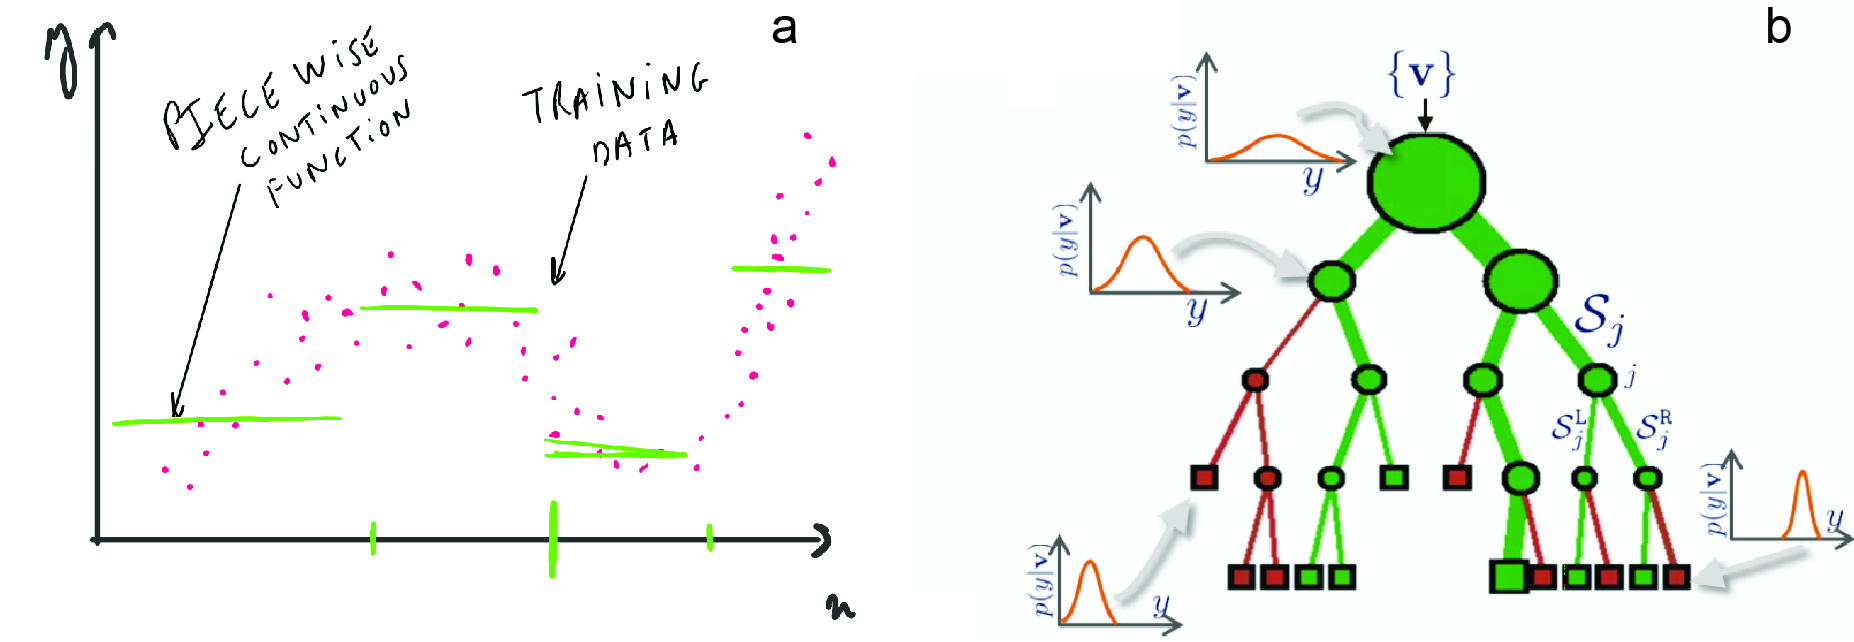
\includegraphics[width=1\textwidth]{rf}
	\caption{Detail of a regression forest - (a) the continuous data is approximated by a piecewise continuous function. The subdivision of the x interval stops when the entropy or SSE has reached a threshold value - (b) an example of regression tree from 	\cite{criminisi2011decision}, the leaves of the tree determine values of continuous outputs for subdomains of x}
	\label{fig:rf}
\end{figure}
\begin{figure}[H]
	\centering
	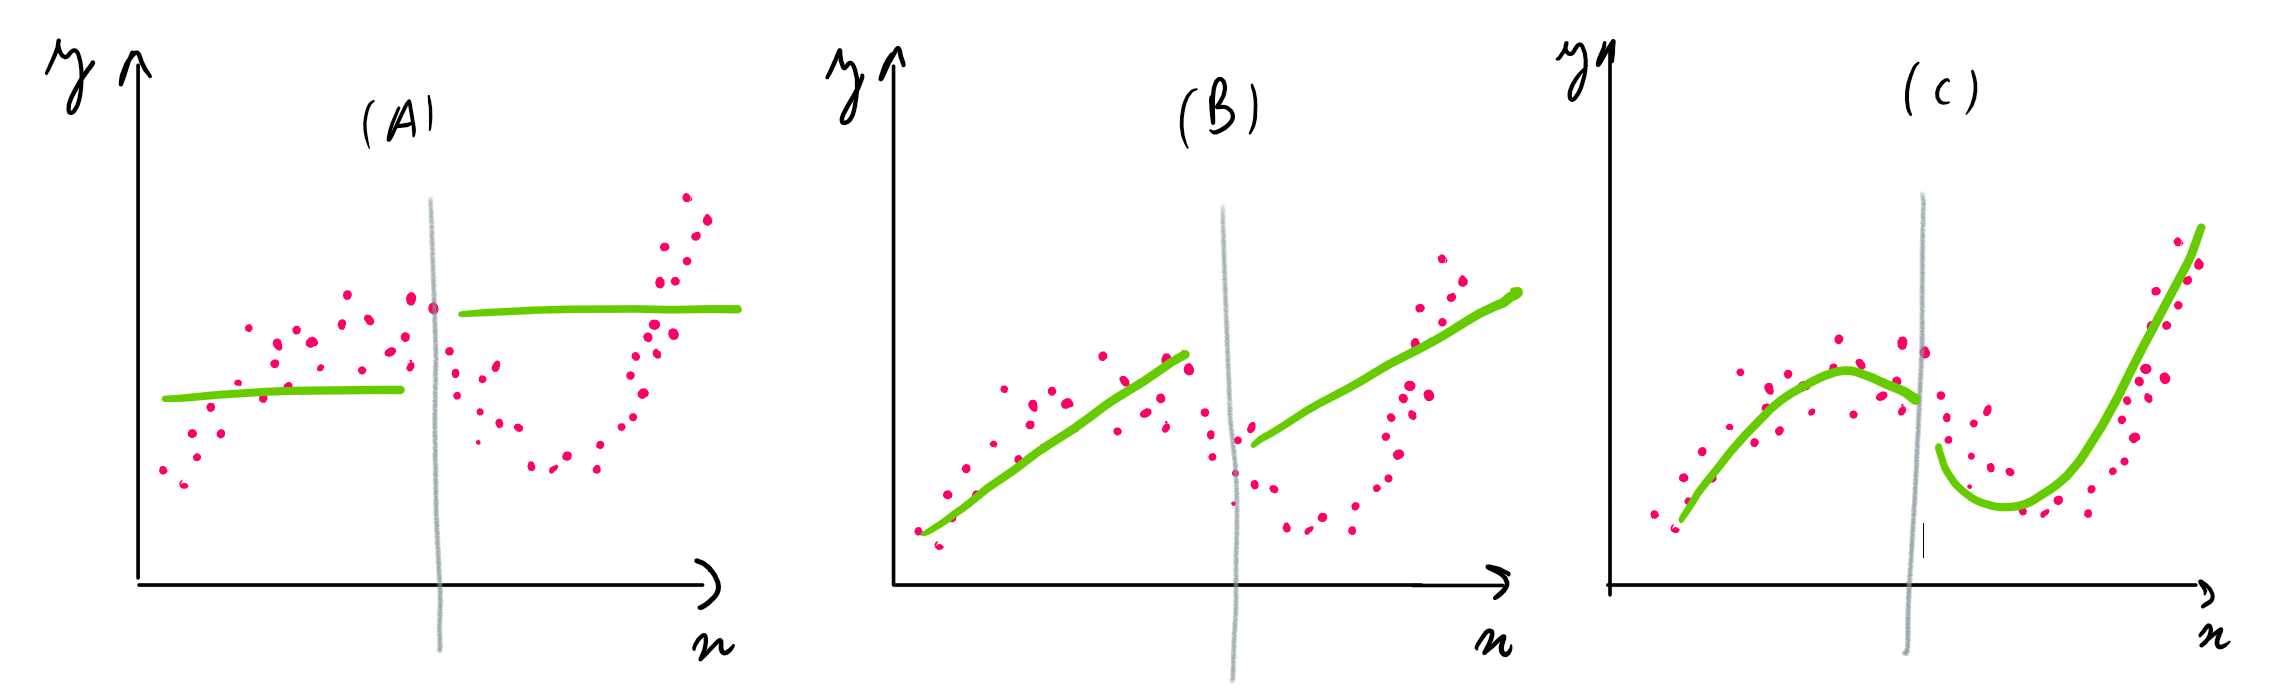
\includegraphics[width=1\textwidth]{rfpredictors}
	\caption{Example of three predictor models (a) constant - (b) linear and (c) polynomial}
	\label{fig:RFpredictors}
\end{figure}
In the case of the constant predictor, the value of the predictor is given by the minimization of the sum of squared error (SSE) as given by Equation \ref{sse_eqn} for the subdomain $D_k$. 
\begin{equation} \label{sse_eqn}
\hat{y}_k = \argmin_y \sum_{i \in D_k} (y-y_i)^2
\end{equation}
Two parameters appears as main control nobs of the method: the number of regression trees in the ensemble and the depth of those trees. Each of those parameter has a distinct effect on the prediction. The depth of the trees controls the closeness of the fit. A ensemble of trees of depth 1 will correspond to a linear regression since each tree corresponds to its root node. In comparison, an ensemble of very deep trees will risk being over-fitted. The number of trees in the forest influences the smoothness of the prediction, the more trees the smoother the direction of the prediction.\\
Two parameters appears as main control nobs of the method: the number of regression trees in the ensemble and the depth of those trees. Each of those parameter has a distinct effect on the prediction. The depth of the trees controls the closeness of the fit. A ensemble of trees of depth 1 will correspond to a linear regression since each tree corresponds to its root node. In comparison, an ensemble of very deep trees will risk being overfitted. The number of trees in the forest influences the smoothness of the prediction, the more trees the smoother the direction of the prediction.\\
Finally regression forest is a preferred method due to its speed, efficiency, ability to cope with missing data and flexibility of use. 
% This is the results section og the report on homework-2.
% Author(s) : Vivek Kumar / Victor Charpentier
% Last Updated : 04/03/2018
%%%%%%%%%%%%%%%%%%%%%%%%%%%
\section{Results and Discussion}

\section{Conclusions}
\vspace*{-10pt}
Based on the results presented above, it can be concluded that RandomForest is the best regression technique for the continuous variables. Feature selection helps but the reduction in the MSE from the cross-validation suggests not such a great increase in accuracy. However, Performing Principal Component Analysis definitely helps in reduction in computation time. As the data-set becomes larger it would be of paramount importance to perform such dimensional reductions.
\section{Bibliography}
\bibliography{ref}
\bibliographystyle{plain}
\end{document}
